 \documentclass[h]{article}
\usepackage[margin=0.5in]{geometry}
\usepackage{amsfonts} 
\usepackage{textcomp}
 
\usepackage{graphicx}
\usepackage{caption}
\usepackage{subcaption}
\usepackage{float} 
\usepackage{flafter}
\graphicspath{ {../images/} }
\usepackage{adjustbox}


\newcommand{\cent}{\textcent \hspace{4pt}}
\title{CS 7641 Machine Learning \\ Assignment 1}
\date{Due February 4th, 2018 11:59pm}
\author{Philip Bale \\ pbale3}

\begin{document}

\maketitle

\section*{Classification Problems}
\subsection*{1) US Permanent Visa Applications}  
\subsubsection*{Overview}
The first classification problem revolves around classifying whether or not a 
person's US permanent visa application will be accepted or denied based on the parameters of 
their application.  Among the features used in the classifcation are:
\begin{itemize}
  \item Job features: Industry code, job class, wage rate, wage type
  \item Geographic features: Country of citizen and employer location
\end{itemize}
The classes observed for this dataset are simply 'approved' and 'denied'.  The 
dataset contains 374365 total samples.
\subsubsection*{Why is the dataset interesting?}
This dataset is interesting due to its potential to aid in the visa application 
process from a cost and time savings potential.  It could also enable confidence in those 
interested in applying for a US permanent visa but doubting their chances of 
acceptance.  At the end of the day, the goal is it to try to determine the application result 
before time, money, and other resources are spent.  As someone who has worked 
with a large number of first-generation visa holders and immigrants, I am 
extremely interested in building tools to help others to achieve the same.
\\ \\
From a machine learning perspective, the dataset is incredibly interesting due 
to its wide variety of features and the variety of values those features can take. 
 An immense number of job types, wage rates, and citizenships alone create an 
 extremely diverse dataset.  Additionally, the number of samples available 
 provide a comprehensive picture of historical data, lending towards greater 
 cofidence in training and testing rates.

\subsection*{2) Home Sale Price Predictions}  
\subsubsection*{Overview}
The second classification problem revolves around classifying a home's price 
bracket based upon the various characteristics of the home.  Among the features 
used in the classification are :
\begin{itemize}
  \item Subjective measurements: Exterior condition, house style, overall quality rating, and overall condition
  \item Objective measurements: Type of dwelling, building type, lot size, neighborhood, year built, and year sold
\end{itemize}
After an initial review of the dataset, the classes were defined as pricing 
brackets divided into 100k groups.  I.e: 0-100k, 100k-200k, 200k-300k, etc.  The 
dataset contains 1451 samples.  An additional dataset containing another 1400 
testing samples exists but was not used as it contains unclassified sale 
prices.  It will, however, prove useful for unsupervised learning.
\subsubsection*{Why is the dataset interesting?}
This dataset is interesting for two primary reasons: real-world applicability 
and participating in a Kaggle challenge.  First, modeling home prices is both a 
difficult and lucrative task.  If one can succesfully model home sale prices on 
large sets of data, he/she can make large amounts of money investing in real 
estate when he/she detects outliers in listed price vs. what it is expected to sell for.  
This applies to flipping, investing, and remodeling.  Second, the dataset is 
part of an ongoing Kaggle competition that does not have a winning solution yet. 
 By taking part of the competition, the dataset presents the opportunity to work 
 towards a winning solution and advance ones algorithms over time. 
 \\ \\
 Houses can have a very large amount of features--with a large amount of variety 
 in the individual features.  Similarly, housing is prone to personal taste and 
 frequent need for upgrades/modernization.  In such, I believe price estimation is an 
 excellent problem, full of depth and complexity, that is suitable for a machine 
 learning approach.
 
  \section*{General Data Processing}
  The datasets I used were both relatively clean to begin with.  One small 
  problem, however, was that a lot of my features on both datasets were 
  text-based.  To transform the features into numeric values suitable for the 
  machine learning algorithms, I used a label encoder built into ScikitLearn.
  \\ \\
  I also did a small amount of preprocessing of the data to make it more 
  suitable for classification.  I dropped all unnecessary columns to help 
  speed up with data processing in general--which proved immensely helpful when 
  dealing with the more computationall intensive algorithms.  In the 
  case of home prices, I precalculated the brackets based on the 'sale price' data label.  
  In the case of visa applications, I pregrouped the case outcome so that 
  results such as 'certified' and 'certified withdrawn' are both concerned as 
  'approved' conditions whereas 'denied', 'invalidated', and 'rejected' all 
  resolve to 'denied'.
  
 \section*{#1: Decision Trees}
 A decision tree classifier was the first algorithm applied to the datasets.  
 Various values of max\_depth were tested as a means of pruning unnecessary 
 leaves.  Similarly, a grid search was used to test whether a 'gini' or 
 'entropy' criterion was more effective.

\subsection*{US Permanent Visa Data}
\begin{figure}[H]
\minipage{0.69\textwidth}
\begin{tabular}{ | c | c  | c | c | c | c | c |} 
\hline
\textbf{Depth} & \textbf{Criterion} & \textbf{Tree Size} & \textbf{Train \%} & \textbf{Train Time} & \textbf{Test \%} & \textbf{Test Time}   \\
\hline
1 & gini & 3 & 0.7657 & 0.1212 & 0.7680 & 0.0010 \\ \hline
3 & gini & 15 & 0.6775 & 0.1417 & 0.6749 & 0.0009 \\ \hline
6 & entropy & 105 & 0.7121 & 0.2605 & 0.6924 & 0.0011 \\ \hline
10 & gini & 889 & 0.7584 & 0.3192 & 0.7072 & 0.0011 \\ \hline
15 & gini & 3013 & 0.8628 & 0.4199 & 0.7582 & 0.0014 \\ \hline
20 & gini & 4751 & 0.9299 & 0.4517 & 0.7917 & 0.0010 \\ \hline
25 & gini & 5349 & 0.9545 & 0.5284 & 0.8032 & 0.0010 \\ \hline
35 & entropy & 5349 & 0.9574 & 0.5116 & 0.8081 & 0.0010 \\ \hline
\end{tabular}
\caption*{Results at multiple depths for best criterion via grid search}
\endminipage\hfill
\minipage{0.29\textwidth}
\begin{flushright}
\begin{tabular}{ | c | c | c  | } 
\hline
 & Accepted & Denied  \\
\hline
Accepted & 96 & 135 \\ \hline
Denied & 217 & 1376 \\ \hline
\end{tabular}
\caption*{Test Data Confusion matrix}
\end{flushright}
\endminipage\hfill

\end{figure}

\begin{figure}[H]
  \minipage{0.32\textwidth}
      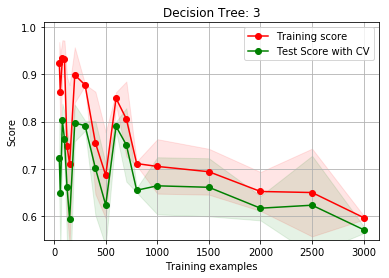
\includegraphics[width=1\textwidth,keepaspectratio]{1_curve_dtree3.png} 
      \caption*{Learning Curve for max\_depth = 3} 
   \endminipage\hfill
   \minipage{0.32\textwidth}
      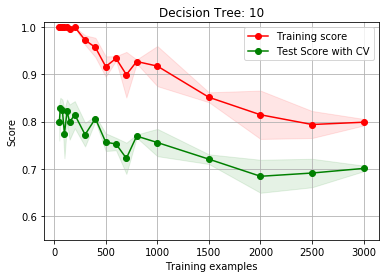
\includegraphics[width=1\textwidth,keepaspectratio]{1_curve_dtree10.png} 
      \caption*{Learning Curve for max\_depth = 10} 
   \endminipage\hfill
   \minipage{0.32\textwidth}
      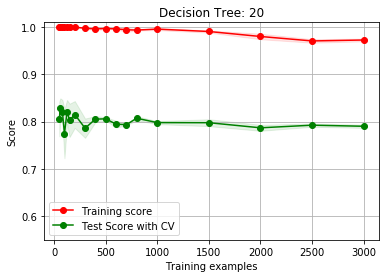
\includegraphics[width=1\textwidth,keepaspectratio]{1_curve_dtree20.png} 
      \caption*{Learning Curve for max\_depth = 20} 
   \endminipage\hfill
\end{figure}

\subsection*{Housing Prices Data}
\begin{figure}[H]
\minipage{0.69\textwidth}
\begin{tabular}{ | c | c  | c | c | c | c | c |} 
\hline
\textbf{Depth} & \textbf{Criterion} & \textbf{TreeSize} & \textbf{Train \%} & \textbf{Train Time} & \textbf{Test \%} & \textbf{Test Time}   \\
\hline
1 & gini & 3 & 0.0912 & 0.0355 & 0.0890 & 0.0006 \\ \hline
3 & entropy & 15 & 0.5816 & 0.0401 & 0.5890 & 0.0003 \\ \hline
6 & entropy & 91 & 0.6820 & 0.0442 & 0.6438 & 0.0003 \\ \hline
10 & gini & 331 & 0.8575 & 0.0566 & 0.6918 & 0.0006 \\ \hline
15 & gini & 593 & 0.9854 & 0.0695 & 0.7603 & 0.0003 \\ \hline
20 & gini & 643 & 1.0000 & 0.0559 & 0.7603 & 0.0007 \\ \hline
25 & gini & 639 & 1.0000 & 0.0550 & 0.7603 & 0.0006 \\ \hline
35 & gini & 639 & 1.0000 & 0.0570 & 0.7603 & 0.0006 \\ \hline

\end{tabular}
\caption*{Results at multiple depths for best criterion via grid search}
\endminipage\hfill
\minipage{0.29\textwidth}
\begin{flushright}
\begin{tabular}{ | c | c | c  | c | c | c | } 
\hline
 & 0-1 & 1-2 & 2-3 & 3-4 & 4-5  \\
\hline
0-1 & 2 & 6 & 0 & 0 & 0 \\ \hline 
1-2 & 4 & 87 & 7 & 0 & 0 \\ \hline 
2-3 & 0 & 8 & 15 & 1 & 2 \\ \hline 
3-4 & 0 & 0 & 6 & 3 & 0 \\ \hline 
4-5 & 0 & 0 & 2 & 0 & 3 \\ \hline 
\end{tabular}
\caption*{  \ \ \  Test Data Confusion matrix  \\  \ \ \ \ \ \ (classes in 100ks)}
\end{flushright}
\endminipage\hfill

\end{figure}

\begin{figure}[H]
  \minipage{0.32\textwidth}
      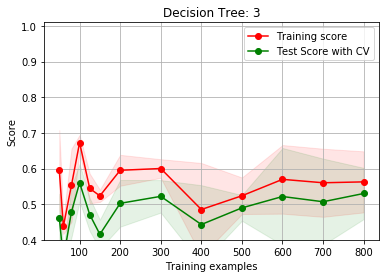
\includegraphics[width=1\textwidth,keepaspectratio]{2_curve_dtree3.png} 
      \caption*{Learning Curve for max\_depth = 3} 
   \endminipage\hfill
   \minipage{0.32\textwidth}
      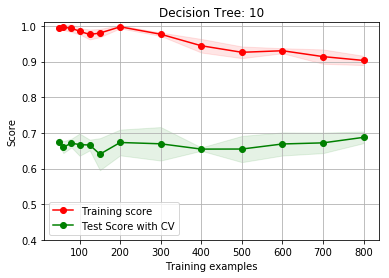
\includegraphics[width=1\textwidth,keepaspectratio]{2_curve_dtree10.png} 
      \caption*{Learning Curve for max\_depth = 10} 
   \endminipage\hfill
   \minipage{0.32\textwidth}
      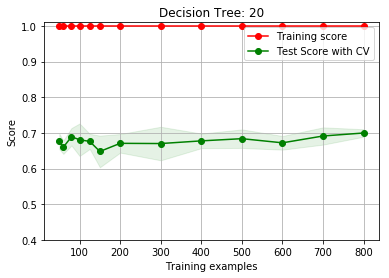
\includegraphics[width=1\textwidth,keepaspectratio]{2_curve_dtree20.png} 
      \caption*{Learning Curve for max\_depth = 20} 
   \endminipage\hfill
\end{figure}

\subsection*{Analysis for Decision Tree}
Overall the classifier worked quite well for both datasets, but was extremely prone to 
overfitting.  Examining the results of the decision tree classifier on the two 
datasets provides numerous observations and basis for analysis, which are provided below.

\subsubsection*{Effects of dataset size & cross validation:}
Above, learning curves are provided for both datasets.  It is immediately 
apparent that the size of the dataset greatly affects the performance of the 
algorithm--though diminishes over time. This makes sense for a few different 
reasons.  The more data we have to train on, the more likely it is that 
we see the full spectrum of possible variability.  Similarly, the broader the 
set of examples, the less biased our algorithm will be.  This is because if we 
only train on a few data samples, then our algorithm can only make decisions 
based on the features learned from the small, simple sample size--thus generating a bias (and therefore 
underfitting).
\\ \\ 
The learning curves for both datasets clearly level out as 
dataset size increases, demonstrating less variance with a more informed model.  
Similarly, cross-validation was used to normalize the training 
samples and smooth the learnign curve.  Without cross-validationg, the model was 
prone to unrepresentative, biased dataset samples during training and, in-turn, testing.
\subsubsection*{Tuning Parameters:}
The two main paremeters tuned were maximum tree depth and the split criterion.  
The split criterion measures the quality of a tree split.  Both 'gini' and 
'entropy' were tested and evaluated using a gridsearch.  For the large majority 
of trials, especially with larger and more complex trees, 'gini' was the more 
effective splitting criterion--though the results for the two were nearly 
identical.  If anything, Gini was more performant due to it's mathematical 
simplicity over the entropy formula.
\\ \\
Tree depth provided to be a singificant influencer over the performance of our 
model--especially for the housing dataset.  By allowing for a greater tree 
depth, we allow for a more complex tree with more possible decisions.  A problem 
emerges when the tree becomes too deep, however.  Instead of becoming more 
robust, the tree begins to overfit with very specific branches for very specific 
data items.  By analyzing the test \% vs. depth tradeoff, we can prune 
unnecessary tree depths for the optimal tree size.  This allowed for both a 
fast, accurate tree with a reasonable footprint.

\subsubsection*{Performance:}
Peformance varied for the two datasets across a few different domains.  In terms of runtime, housing prices took 
longer than the visa data to train (about 10x)--though both were extremely fast on a powerful laptop.
  This was mainly due to a larger dataset size.  As 
the depth of the tree increased, the training time also took longer for both datasets due to the
increased tree size and complexity(as can be seen from the table above).
\\ \\ 
In terms of accuracy, the visa data started out somewhat high but was able to gain about 4\% through 
optimizing the depth of the tree.  This is due to the fact that features like 
'salary' and 'job type' proved to heavily influence the approval process.  The 
housing data, however, saw more greater improvements as depth increased.    As a 
more diverse and variable dataset, the model was able to gain a lot of accuracy 
as the tree grew because it could accommodate more specific feature branches.  While the test data
started out at \textless 10\%, it was able to grow to approximately 76\%.   

\begin{figure}[H]
    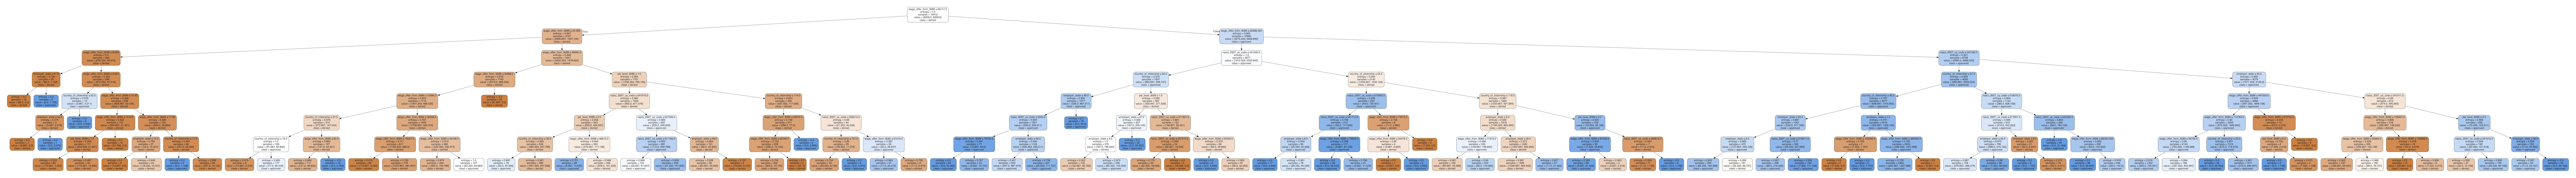
\includegraphics[width=1.0\textwidth,keepaspectratio]{1_dtree.jpg} 
    \caption*{SampleDecision Tree: Permanent Visa with max\_depth of 7} 
\end{figure}

\section*{#2) AdaBoost - Boosted Trees}
A boosted decision tree classifer, Adaboost, was the second algorithm applied.  It used the same 
base decision tree as the first model algorithm.  Based on the results of the 
first model, we decided to stick with 'gini' as the criterion for faster 
training.

\subsection*{US Permanent Visa Data}
\begin{figure}[H]
\minipage{0.69\textwidth}
\begin{tabular}{ | c | c  | c | c | c | c | c |} 
\hline
\textbf{Depth} & \textbf{Learning Rate} & \textbf{\# Estimators} & \textbf{Train \%} & \textbf{Train Time} & \textbf{Test \%} & \textbf{Test Time}   \\
1 & 0.1 & 150 & 0.8705 & 24.1484 & 0.8662 & 0.0327 \\ \hline
3 & 0.1 & 100 & 0.8770 & 39.7266 & 0.8679 & 0.0216 \\ \hline
5 & 0.1 & 5 & 0.8761 & 53.8227 & 0.8706 & 0.0021 \\ \hline
10 & 0.1 & 150 & 0.9775 & 82.2192 & 0.8745 & 0.0504 \\ \hline
15 & 1 & 150 & 0.9775 & 94.5996 & 0.8701 & 0.0420 \\ \hline
20 & 1 & 150 & 0.9775 & 107.0742 & 0.8618 & 0.0452 \\ \hline
\hline
\end{tabular}
\caption*{Results at multiple depths for best learning rate/# estimators via grid search}
\endminipage\hfill
\end{figure}

\begin{figure}[H]
  \minipage{0.32\textwidth}
      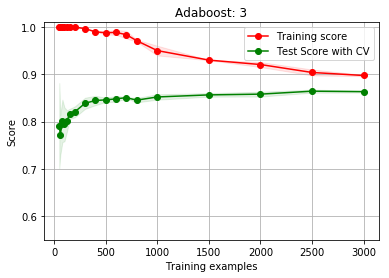
\includegraphics[width=1\textwidth,keepaspectratio]{1_curve_boost3.png} 
      \caption*{Learning Curve for max\_depth = 3} 
   \endminipage\hfill
   \minipage{0.32\textwidth}
      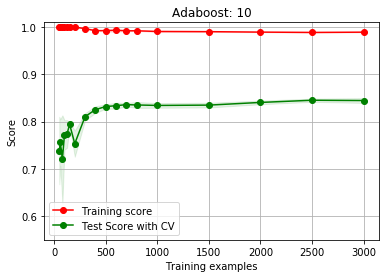
\includegraphics[width=1\textwidth,keepaspectratio]{1_curve_boost10.png} 
      \caption*{Learning Curve for max\_depth = 10} 
   \endminipage\hfill
   \minipage{0.32\textwidth}
      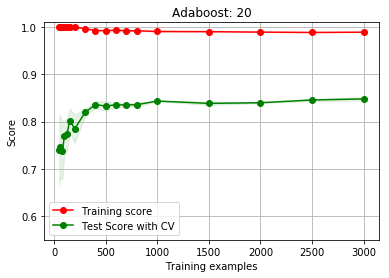
\includegraphics[width=1\textwidth,keepaspectratio]{1_curve_boost20.png} 
      \caption*{Learning Curve for max\_depth = 20} 
   \endminipage\hfill
\end{figure}

\subsection*{Housing Prices Data}
\begin{figure}[H]
\minipage{0.69\textwidth}
\begin{tabular}{ | c | c  | c | c | c | c | c |} 
\hline
\textbf{Depth} & \textbf{Learning Rate} & \textbf{\# Estimators} & \textbf{Train \%} & \textbf{Train Time} & \textbf{Test \%} & \textbf{Test Time}   \\
\hline
1 & 0.1 & 15 & 0.6881 & 6.9413 & 0.6918 & 0.0018 \\ \hline
3 & 0.1 & 5 & 0.7724 & 8.2909 & 0.7945 & 0.0013 \\ \hline
5 & 0.1 & 3 & 0.8291 & 10.8559 & 0.7740 & 0.0011 \\ \hline
10 & 1 & 50 & 1.0000 & 13.6713 & 0.7945 & 0.0057 \\ \hline
15 & 1 & 100 & 1.0000 & 8.7526 & 0.8014 & 0.0145 \\ \hline
20 & 0.1 & 15 & 1.0000 & 0.6862 & 0.6781 & 0.0009 \\ \hline

\end{tabular}
\caption*{Results at multiple depths for best learning rate/# estimators via grid search}
\endminipage\hfill

\end{figure}

\begin{figure}[H]
  \minipage{0.32\textwidth}
      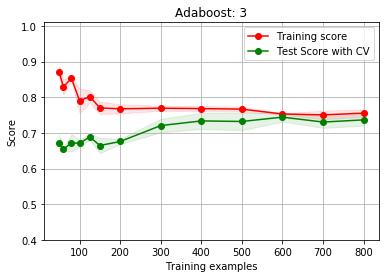
\includegraphics[width=1\textwidth,keepaspectratio]{2_curve_boost3.png} 
      \caption*{Learning Curve for max\_depth = 3} 
   \endminipage\hfill
   \minipage{0.32\textwidth}
      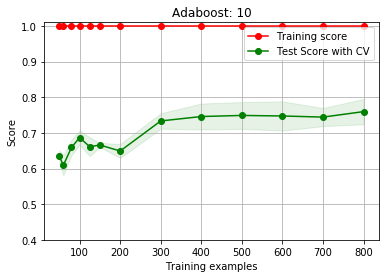
\includegraphics[width=1\textwidth,keepaspectratio]{2_curve_boost10.png} 
      \caption*{Learning Curve for max\_depth = 10} 
   \endminipage\hfill
   \minipage{0.32\textwidth}
      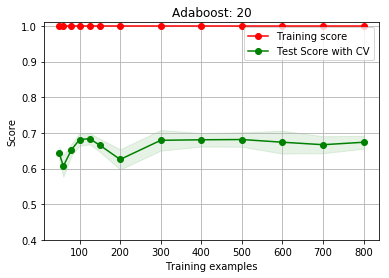
\includegraphics[width=1\textwidth,keepaspectratio]{2_curve_boost20.png} 
      \caption*{Learning Curve for max\_depth = 20} 
   \endminipage\hfill
\end{figure}

\subsection*{Analysis for AdaBoost Boosted Tree}
The AdaBoost boosted tree relates significantly to the original decision tree 
classifier.  It even uses the decision tree as its base classifier.  The main 
difference, however, exists in the boosting.  As discussed in class, a boosted 
tree is essentially an ensemble of weaker trees.  This ensemble works to 
classify with greater accuracy than the original, simplified tree. 
\\ \\
Evaluating the performance in the chart and graphs above, it is quickly noticed that the AdaBoost tree works
significantly better for both datasets.  For visa applications, it is approximately 7\% better in the optimal 
configuration.  For housing prices, it i approximately 4\% better.  Training 
times take signifcantly longer, which makes sense as the algorithm trains a much 
larger, ensemble classifier.  For example, the larger permanent visa dataset took more than a minute to
 train for depths greater than 5--compared to less than a second for a normal 
 tree classifier.
 \\ \\
 In terms of parameters, learning rate, depth, and # of estimators were all 
 tuned using a gridsearch to find an optimal model.  As # of estimators 
 increased, optimal learning rate tended to increase too.  For a deeper tree, 
 fewer estimators were needed because the optimal learning rate was achieved 
 sooner.  The learning rate, which effects the rate of contribution for each 
 classifier, was optimized between 0.1 and 1, where the learning rate trended 
 higher for deeper trees.
 \\ \\
 While both types of trees peformed well on the datasets, AdaBoost performed 
 exceptionally well.  I believe this is due to the rich set of features and logically 
 classifiable outcomes.  The AdaBoosted tree still overclassified at 
 increased depth.  By pruning depth to approximately 10 to 15, we were able to achieve 
 an optimal tree.
 
 \section*{#3) Neural Networks}
A neural network (using ScikitLearn's multi-layer perceptron classifier) was the third algorithm applied.  
A combination of different solvers, learning rates, and scaling was used to 
observe the functionality of the networks in regards to our dataset.


\begin{figure}[H]
  \minipage{0.49\textwidth}
      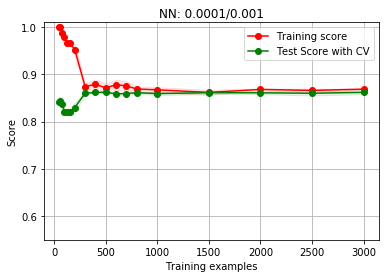
\includegraphics[width=1\textwidth,keepaspectratio]{1_nn.png} 
      \caption*{Permanent Visa Applicant NN Learning Curve} 
   \endminipage\hfill
   \minipage{0.49\textwidth}
      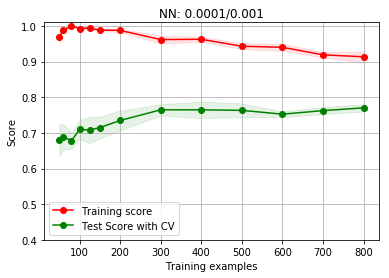
\includegraphics[width=1\textwidth,keepaspectratio]{2_nn.png} 
      \caption*{Housing Price NN Learning Curve} 
   \endminipage\hfill
\end{figure}

\begin{figure}[H]
  \minipage{1\textwidth}
      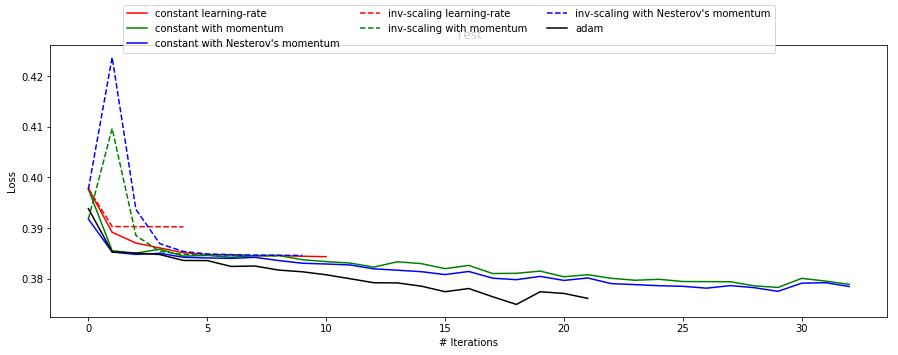
\includegraphics[width=1\textwidth,keepaspectratio]{1_nn_together.png} 
      \caption*{Permanent Visa Applicant NN Configurations Loss Curve} 
   \endminipage\hfill
   \minipage{1\textwidth}
      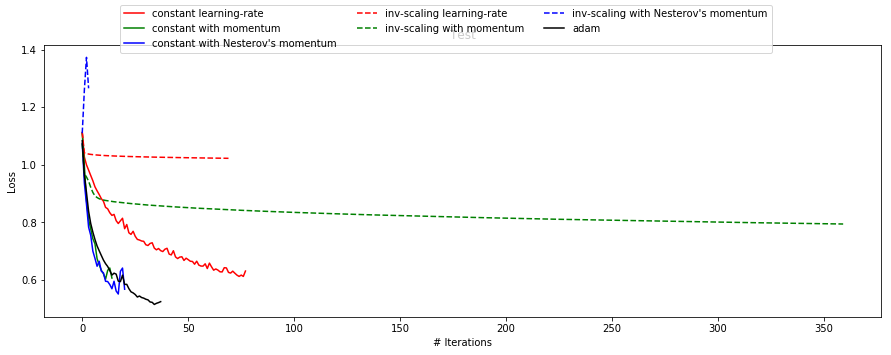
\includegraphics[width=1\textwidth,keepaspectratio]{2_nn_together.png} 
      \caption*{Housing Price NN Configurations Loss Curve} 
   \endminipage\hfill
\end{figure}

\begin{figure}[H]
\minipage{0.69\textwidth}
\begin{tabular}{ | c | c  | c | c | c | c | c |} 
\hline
\textbf{NN Config} & \textbf{Test Score} & \textbf{Loss} & \textbf{Train Time}   \\ 
\hline
constant learning-rate & 0.8642 & 0.3842 & 0.6121 \\ \hline
sgd constant  learning-rate with momentum & 0.8663 & 0.3823 & 0.7120 \\ \hline
sgd constant  learning-rate with Nesterov's momentum & 0.8668 & 0.3779 & 1.4836 \\ \hline
sgd inv-scaling learning-rate & 0.8646 & 0.3905 & 0.2435 \\ \hline
sgd inv-scaling with momentum & 0.8646 & 0.3842 & 0.3750 \\ \hline
sgd inv-scaling with Nesterov's momentum & 0.8646 & 0.3848 & 0.2740 \\ \hline
adam constant  learning-rate & 0.8677 & 0.3650 & 2.1166 \\ \hline
\end{tabular}
\caption*{Permanent Visa results for various NN configs}
\endminipage\hfill
\end{figure}

\begin{figure}[H]
\minipage{0.69\textwidth}
\begin{tabular}{ | c | c  | c | c | c | c | c |} 
\hline
\textbf{NN Config} & \textbf{Test Score} & \textbf{Loss} & \textbf{Train Time}   \\ 
\hline
sgd constant learning-rate & 0.7664 & 0.6301 & 0.4272  \\ \hline
sgd constant learning-rate with momentum & 0.7498 & 0.6058 & 0.0889 \\ \hline
sgd constant  learning-ratewith Nesterov's momentum & 0.7595 & 0.5669 & 0.1286 \\ \hline
sgd inv-scaling learning-rate & 0.6278 & 1.0219 & 0.3932  \\ \hline
sgd inv-scaling with momentum & 0.7009 & 0.7936 & 1.9339  \\ \hline
sgd inv-scaling with Nesterov's momentum & 0.6278 & 1.2652 & 0.0205  \\ \hline
adam constant  learning-rate  & 0.7795 & 0.5237 & 0.2093  \\ \hline
\end{tabular}
\caption*{Housing Price results for various NN configs}
\endminipage\hfill
\end{figure}

\subsection*{Analysis for Neural Networks}
The neural network models, while effective, performed slightly worse 
than the boosted decision tree.  After preliminary exploration, it became 
apparent that the wide variety of neural network configurations performed 
differently depending on the given  dataset.
\\ \\
In terms of training and testing, cross-validation was used to ensure a robust 
sampling.  The housing price dataset started to converge slowly in regards to 
the learning curve, whereas the permanent visa dataste convered very rapidly.  
The permanent visa dataset, by converging rapidly, showed it's low variability.  
The network model was able to very quickly learn the features--in less than 40--though its feature set is
 smaller than those of the housing prices.  The housing price dataset, 
 conversely, required many more iterations to learn.  
 \\ \\
 Various neural network configurations were used on the test data.  Configurations were created by 
 varying the weight optimizer, learning-rate, momentum, and scaling.  To aid 
 with speed and peformance, a pre-process Scaler was applied to the datasets.
 Additionally, a gridsearch approach was applied with various alpha, learning 
 rate, solver, and hidden layer conigurations.  While complete results achieved by the various networks are listed
  above, below we will look at the top performing network for each dataset to try to 
  understand why it was most effective.
  \\ \\
  For the permanent visa dataset, practically every algorithm performed the same.  At first, this perplexed me, 
  as I expected that at least different learning rates and solvers would create 
  different results.  It turns out, however, for a dataset that is more easily 
  learnable and converges on fewer iterations, this makes sense.  It takes less 
  effort and hyperparemeterization to find functional solutions.  To verify that 
  my results were accurate, I also ran a gridsearched neural network with a 2000 
  iteration limit and various values of solver, learning\_rate, and hidden 
  layers.
  \\ \\
  For the housing price dataset, the 'adam' weight optimizer significantly outperformed the others.  
  This was quite different than the Permanent Visa dataset, which performed 
  rather homogenously.  The 'adam' optimizer, or solver, is a 'stochastic 
  gradient-based optimizer.' (From SciKit learn manual)  It is noted to work 
  especially well for large datasets.  The learning rate was slightly smaller 
  for this configuration, starting with an initial value of 0.01.   Since the 
  housing price network took longer to converge and performed quite differently 
  for the various configuration, it is reasonable to believe that with a larger 
  dataset, a more complex and accurate network could be trained.  While this 
  would increase training time, the trade off of increased accuracy and lower 
  variance would likely be possible.

 \section*{#4) Support Vector Machines}
Support Vector Machines were the fourth algorithm applied. 

\subsection*{US Permanent Visa Data}

\begin{figure}[H]
\minipage{0.69\textwidth}
\begin{tabular}{ | c | c  | c | c | c | c | c |} 
\hline
\textbf{Kernel} & \textbf{Gamma} & \textbf{Train \%} & \textbf{Train Time} & \textbf{Test \%} & \textbf{Test Time}   \\ \hline
rbf & 0.01 & 0.8642 & 20.4459 & 0.8712 & 0.1536 \\ \hline
rbf & 0.05 & 0.8646 & 29.0756 & 0.8712 & 0.1817 \\ \hline
rbf & 1.0 & 0.8752 & 29.7723 & 0.8745 & 0.1805 \\ \hline
rbf & 2.0 & 0.8798 & 28.6184 & 0.8728 & 0.1914 \\ \hline
poly & 0.01 & 0.8642 & 9.3467 & 0.8712 & 0.0884 \\ \hline
poly & 0.05 & 0.8645 & 20.6110 & 0.8712 & 0.0857 \\ \hline
poly & 1.0 & 0.8301 & 24.1879 & 0.8262 & 0.1198 \\ \hline
poly & 2.0 & 0.8349 & 19.5531 & 0.8355 & 0.0391 \\ \hline

\hline
\end{tabular}
\caption*{Permanent Visa Data for various kernel/gamma configurations}
\endminipage\hfill
\end{figure}

\begin{figure}[H]
  \minipage{0.32\textwidth}
      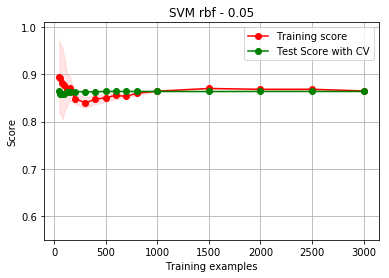
\includegraphics[width=1\textwidth,keepaspectratio]{1_svm_rbf_05.png} 
      \caption*{RBF SVM w/ 0.05 gamma} 
   \endminipage\hfill
   \minipage{0.32\textwidth}
      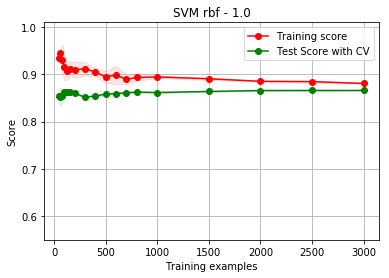
\includegraphics[width=1\textwidth,keepaspectratio]{1_svm_rbf_1.png} 
      \caption*{RBF SVM w/ 1.0 gamma} 
   \endminipage\hfill
   \minipage{0.32\textwidth}
      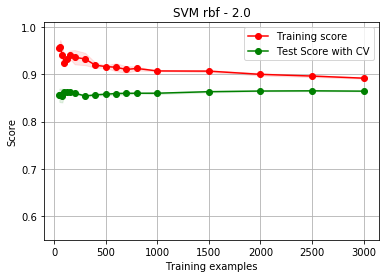
\includegraphics[width=1\textwidth,keepaspectratio]{1_svm_rbf_2.png} 
      \caption*{RBF SVM w/ 2.0 gamma} 
   \endminipage\hfill
\end{figure}

\begin{figure}[H]
  \minipage{0.32\textwidth}
      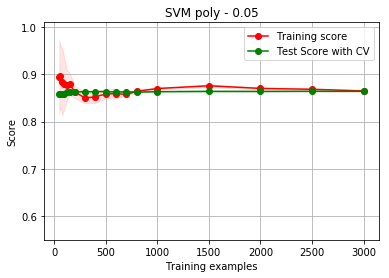
\includegraphics[width=1\textwidth,keepaspectratio]{1_svm_poly_05.png} 
      \caption*{Poly SVM w/ 0.05 gamma} 
   \endminipage\hfill
   \minipage{0.32\textwidth}
      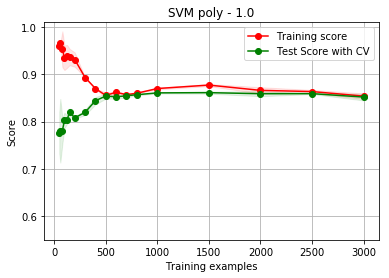
\includegraphics[width=1\textwidth,keepaspectratio]{1_svm_poly_1.png} 
      \caption*{Poly SVM w/ 1.0 gamma} 
   \endminipage\hfill
   \minipage{0.32\textwidth}
      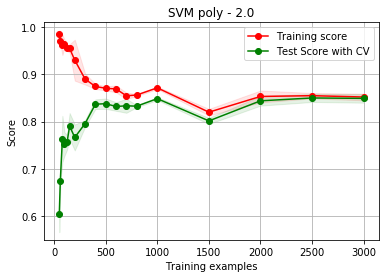
\includegraphics[width=1\textwidth,keepaspectratio]{1_svm_poly_2.png} 
      \caption*{Poly SVM w/ 2.0 gamma} 
   \endminipage\hfill
\end{figure}

\subsection*{Housing Price Data}

\begin{figure}[H]
\minipage{0.69\textwidth}
\begin{tabular}{ | c | c  | c | c | c | c | c |} 
\hline
\textbf{Kernel} & \textbf{Gamma} & \textbf{Train \%} & \textbf{Train Time} & \textbf{Test \%} & \textbf{Test Time}   \\ \hline
rbf & 0.01 & 0.7487 & 0.2301 & 0.7603 & 0.0042 \\ \hline
rbf & 0.05 & 0.7954 & 0.2031 & 0.8219 & 0.0086 \\ \hline
rbf & 1.0 & 0.9226 & 0.5629 & 0.7740 & 0.0042 \\ \hline
rbf & 2.0 & 0.9502 & 0.5996 & 0.7397 & 0.0051 \\ \hline
poly & 0.01 & 0.6276 & 0.1581 & 0.6438 & 0.0024 \\ \hline
poly & 0.05 & 0.7333 & 0.1733 & 0.7534 & 0.0028 \\ \hline
poly & 1.0 & 0.9333 & 0.7254 & 0.7192 & 0.0019 \\ \hline
poly & 2.0 & 0.9280 & 1.0244 & 0.6781 & 0.0019 \\ \hline


\hline
\end{tabular}
\caption*{Housing Price Data for various kernel/gamma configurations}
\endminipage\hfill
\end{figure}

\begin{figure}[H]
  \minipage{0.32\textwidth}
      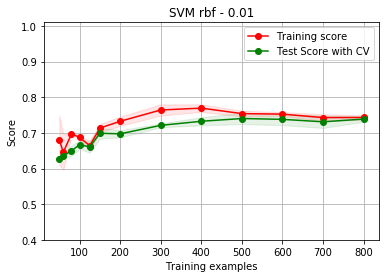
\includegraphics[width=1\textwidth,keepaspectratio]{2_svm_rbf_01.png} 
      \caption*{RBF SVM w/ 0.01 gamma} 
   \endminipage\hfill
   \minipage{0.32\textwidth}
      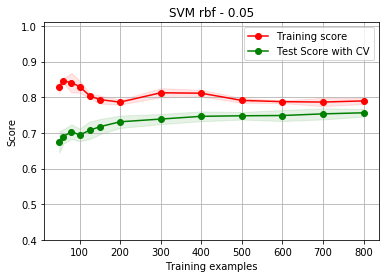
\includegraphics[width=1\textwidth,keepaspectratio]{2_svm_rbf_05.png} 
      \caption*{RBF SVM w/ 0.05 gamma} 
   \endminipage\hfill
   \minipage{0.32\textwidth}
      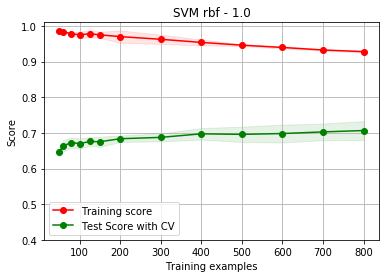
\includegraphics[width=1\textwidth,keepaspectratio]{2_svm_rbf_1.png} 
      \caption*{RBF SVM w/ 1.0 gamma} 
   \endminipage\hfill
\end{figure}
\begin{figure}[H]
  \minipage{0.32\textwidth}
      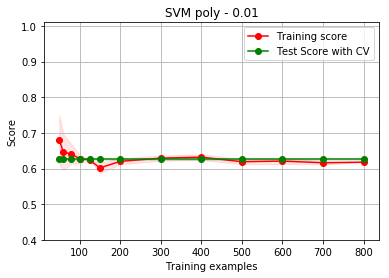
\includegraphics[width=1\textwidth,keepaspectratio]{2_svm_poly_01.png} 
      \caption*{Poly SVM w/ 0.01 gamma} 
   \endminipage\hfill
   \minipage{0.32\textwidth}
      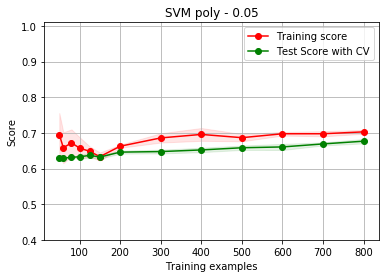
\includegraphics[width=1\textwidth,keepaspectratio]{2_svm_poly_05.png} 
      \caption*{Poly SVM w/ 0.05 gamma} 
   \endminipage\hfill
   \minipage{0.32\textwidth}
      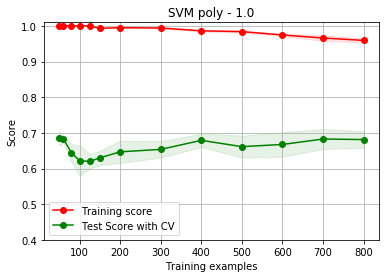
\includegraphics[width=1\textwidth,keepaspectratio]{2_svm_poly_1.png} 
      \caption*{Poly SVM w/ 1.0 gamma} 
   \endminipage\hfill
\end{figure}


\subsection*{Analysis for Support Vector Machines}
The Support Vector Machines peformed well compared to the other algorithms, 
though, on-average, took significantly longer to train.  Overall, the optimal configurations yieled a testing rate of 87.5\% for the 
permanent visa data and 77.4\% for the housing price data.     As there were a lot of 
parameters to tune, a gridsearch was used yet again along with cross-validation 
to ensure a robust and effective model.  The primary parameters were kernel and 
gamma.
\\ \\
To begin, two different  kernels were used for each dataset: 'rbf' and 'poly'.  
For both datasets, the rbf kernel proved more effective.  The gaussian rbf 
kernel essentially calculates squared distance between feature vectors and is 
scaled by gamma.  While the poly kernel tends to overfit the training data, rbf 
does a much better job at securing a robust fit.  To tune Gamma, values on a 
spectrum from 0.01 to 2.0 were used (and results detailed above).
\\ \\
Training time increased signficantly, especially for larger datasets.  Since a 
SVMs require a large amount of iterations and  recalculation to converge to an 
optimal solution, this made sense.  It was especially apparent for the larger 
dataset of permanent visa data.  The training time took approximately 30 seconds 
for the various configurations where as the smaller housing price dataset took 
less than a second on average.
\\ \\
From the learning curves, we see that a highly succesful training rate leads to 
greater overfitting.  This makes sense, as the SVM becomes too rigid to the 
input data, and is not robust.  Similarly, when the kernel has too low of a 
gamma and does not accomodate feature relations properly, the model underfits 
and performs poorly on both training and test data.

 \section*{#5) K-nearest Neighbors}
K-nearest Neighbors was the fifth algorithm applied. 

\subsection*{Permanent Visa Data}

\begin{figure}[H]
\minipage{0.6\textwidth}
\begin{tabular}{ | c | c  | c | c | c | c | c |} 
\hline

\textbf{Weight} & \textbf{K} & \textbf{Train \%} & \textbf{Train Time} & \textbf{Test \%} & \textbf{Test Time}   \\ \hline
uniform & 1 & 0.9708 & 0.3422 & 0.8158 & 0.0080 \\ \hline
uniform & 2 & 0.8978 & 0.3619 & 0.7708 & 0.0094 \\ \hline
uniform & 3 & 0.8989 & 0.3603 & 0.8394 & 0.0106 \\ \hline
uniform & 4 & 0.8854 & 0.3836 & 0.8202 & 0.0103 \\ \hline
uniform & 5 & 0.8892 & 0.3996 & 0.8503 & 0.0107 \\ \hline
uniform & 10 & 0.8742 & 0.4736 & 0.8525 & 0.0126 \\ \hline
uniform & 15 & 0.8739 & 0.5735 & 0.8640 & 0.0134 \\ \hline
uniform & 20 & 0.8738 & 0.6083 & 0.8673 & 0.0168 \\ \hline
uniform & 30 & 0.8696 & 0.8306 & 0.8662 & 0.0219 \\ \hline
uniform & 50 & 0.8686 & 1.1392 & 0.8618 & 0.0315 \\ \hline
distance & 1 & 0.9708 & 0.2706 & 0.8158 & 0.0071 \\ \hline
distance & 2 & 0.9675 & 0.4111 & 0.8103 & 0.0113 \\ \hline
distance & 3 & 0.9743 & 0.4050 & 0.8279 & 0.0096 \\ \hline
distance & 4 & 0.9741 & 0.3766 & 0.8311 & 0.0092 \\ \hline
distance & 5 & 0.9756 & 0.4084 & 0.8377 & 0.0157 \\ \hline
distance & 10 & 0.9762 & 0.4899 & 0.8470 & 0.0142 \\ \hline
distance & 15 & 0.9767 & 0.6011 & 0.8509 & 0.0169 \\ \hline
distance & 20 & 0.9782 & 0.6799 & 0.8591 & 0.0290 \\ \hline
distance & 30 & 0.9782 & 0.9327 & 0.8624 & 0.0255 \\ \hline
distance & 50 & 0.9782 & 1.2837 & 0.8635 & 0.0397 \\ \hline

\hline
\end{tabular}
\caption*{Permanent Visa Data}
\endminipage\hfill
  \minipage{0.45\textwidth}
      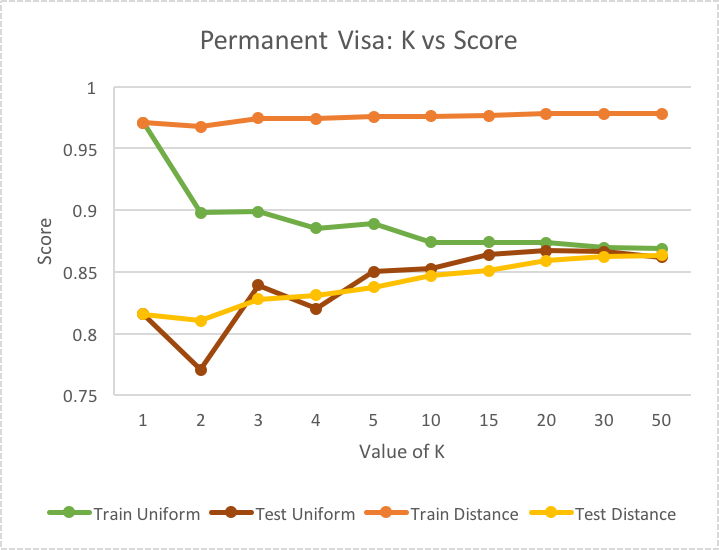
\includegraphics[width=1\textwidth,keepaspectratio]{1_knn_compare.png} 
      \caption*{KNN Comparision} 
   \endminipage\hfill
\end{figure}
 

\begin{figure}[H]
  \minipage{0.32\textwidth}
      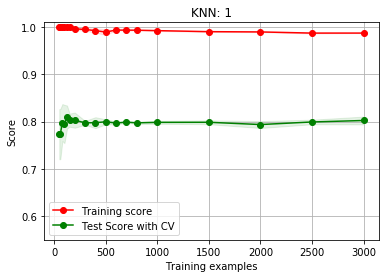
\includegraphics[width=1\textwidth,keepaspectratio]{1_knn_1_1.png} 
      \caption*{Uniform KNN - 1} 
   \endminipage\hfill
   \minipage{0.32\textwidth}
      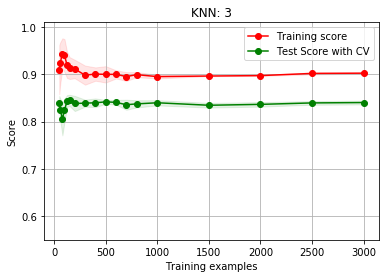
\includegraphics[width=1\textwidth,keepaspectratio]{1_knn_3_1.png} 
      \caption*{Uniform KNN - 3} 
   \endminipage\hfill
   \minipage{0.32\textwidth}
      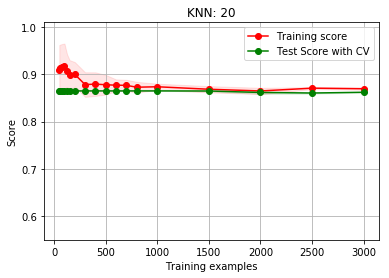
\includegraphics[width=1\textwidth,keepaspectratio]{1_knn_20_1.png} 
      \caption*{Uniform KNN - 20} 
   \endminipage\hfill
\end{figure}
\begin{figure}[H]
  \minipage{0.32\textwidth}
      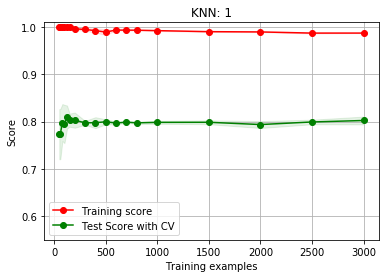
\includegraphics[width=1\textwidth,keepaspectratio]{1_knn_1_2.png} 
      \caption*{Distance KNN - 1} 
   \endminipage\hfill
   \minipage{0.32\textwidth}
      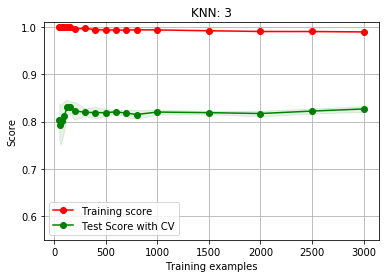
\includegraphics[width=1\textwidth,keepaspectratio]{1_knn_3_2.png} 
      \caption*{Distance KNN - 3} 
   \endminipage\hfill
   \minipage{0.32\textwidth}
      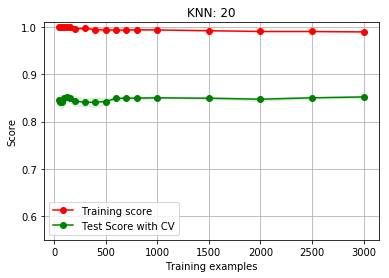
\includegraphics[width=1\textwidth,keepaspectratio]{1_knn_20_2.png} 
      \caption*{Distance KNN - 20} 
   \endminipage\hfill
\end{figure}

\subsection*{Housing Price Data}

\begin{figure}[H]
\minipage{0.6\textwidth}
\begin{tabular}{ | c | c  | c | c | c | c | c |} 
\hline

\textbf{Weight} & \textbf{K} & \textbf{Train \%} & \textbf{Train Time} & \textbf{Test \%} & \textbf{Test Time}   \\ \hline
uniform & 1 & 1.0000 & 0.0343 & 0.6507 & 0.0015 \\ \hline
uniform & 2 & 0.8222 & 0.0304 & 0.6644 & 0.0011 \\ \hline
uniform & 3 & 0.8130 & 0.0283 & 0.7055 & 0.0011 \\ \hline
uniform & 4 & 0.7824 & 0.0379 & 0.6986 & 0.0012 \\ \hline
uniform & 5 & 0.7602 & 0.0351 & 0.7260 & 0.0012 \\ \hline
uniform & 10 & 0.7341 & 0.0324 & 0.7055 & 0.0019 \\ \hline
uniform & 15 & 0.7218 & 0.0369 & 0.7192 & 0.0016 \\ \hline
uniform & 20 & 0.7134 & 0.0466 & 0.7329 & 0.0013 \\ \hline
uniform & 30 & 0.7004 & 0.0488 & 0.7055 & 0.0022 \\ \hline
uniform & 50 & 0.6812 & 0.0635 & 0.6986 & 0.0020 \\ \hline
distance & 1 & 1.0000 & 0.0244 & 0.6507 & 0.0009 \\ \hline
distance & 2 & 1.0000 & 0.0261 & 0.6575 & 0.0010 \\ \hline
distance & 3 & 1.0000 & 0.0293 & 0.7055 & 0.0010 \\ \hline
distance & 4 & 1.0000 & 0.0282 & 0.6986 & 0.0010 \\ \hline
distance & 5 & 1.0000 & 0.0346 & 0.7397 & 0.0011 \\ \hline
distance & 10 & 1.0000 & 0.0356 & 0.7123 & 0.0012 \\ \hline
distance & 15 & 1.0000 & 0.0385 & 0.7192 & 0.0017 \\ \hline
distance & 20 & 1.0000 & 0.0468 & 0.7534 & 0.0021 \\ \hline
distance & 30 & 1.0000 & 0.0501 & 0.7260 & 0.0016 \\ \hline
distance & 50 & 1.0000 & 0.0742 & 0.7055 & 0.0021 \\ \hline

\hline
\end{tabular}
\caption*{Housing Price Data}
\endminipage\hfill
  \minipage{0.45\textwidth}
      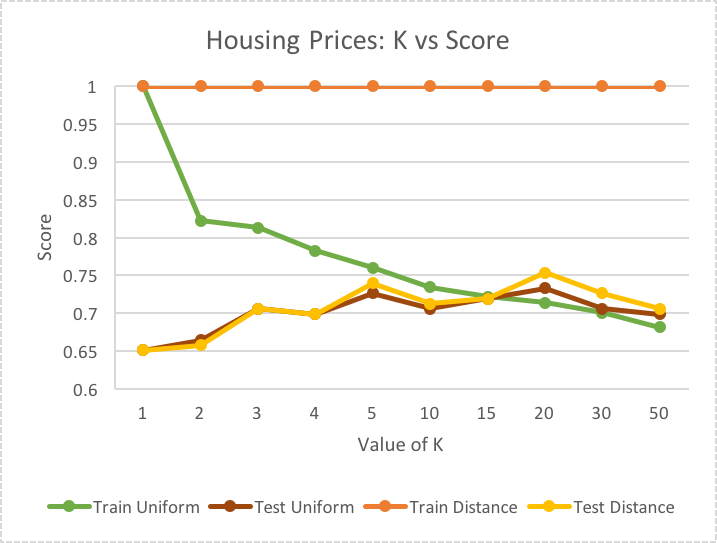
\includegraphics[width=1\textwidth,keepaspectratio]{2_knn_compare.png} 
      \caption*{KNN Comparision} 
   \endminipage\hfill
\end{figure}
 

\begin{figure}[H]
  \minipage{0.32\textwidth}
      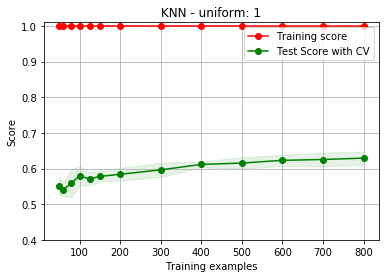
\includegraphics[width=1\textwidth,keepaspectratio]{2_knn_1_1.png} 
      \caption*{Uniform KNN - 1} 
   \endminipage\hfill
   \minipage{0.32\textwidth}
      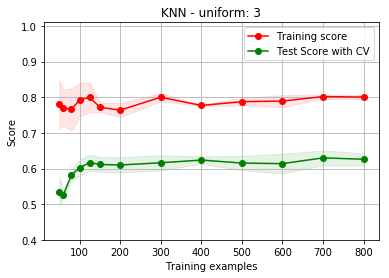
\includegraphics[width=1\textwidth,keepaspectratio]{2_knn_3_1.png} 
      \caption*{Uniform KNN - 3} 
   \endminipage\hfill
   \minipage{0.32\textwidth}
      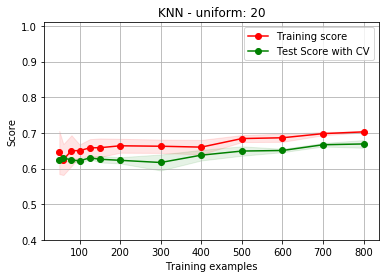
\includegraphics[width=1\textwidth,keepaspectratio]{2_knn_20_1.png} 
      \caption*{Uniform KNN - 20} 
   \endminipage\hfill
\end{figure}
\begin{figure}[H]
  \minipage{0.32\textwidth}
      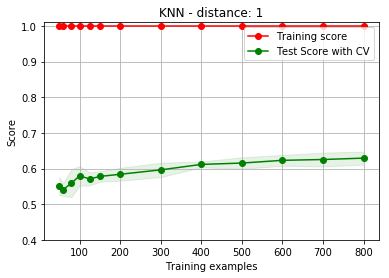
\includegraphics[width=1\textwidth,keepaspectratio]{2_knn_1_2.png} 
      \caption*{Distance KNN - 1} 
   \endminipage\hfill
   \minipage{0.32\textwidth}
      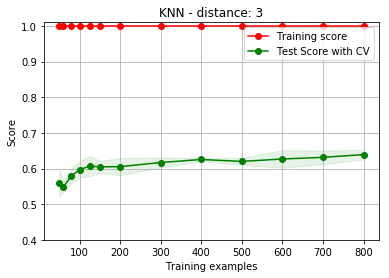
\includegraphics[width=1\textwidth,keepaspectratio]{2_knn_3_2.png} 
      \caption*{Distance KNN - 3} 
   \endminipage\hfill
   \minipage{0.32\textwidth}
      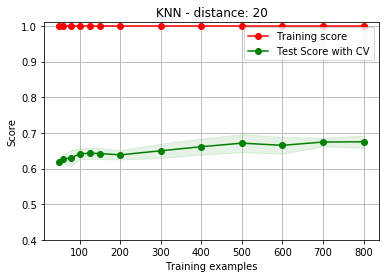
\includegraphics[width=1\textwidth,keepaspectratio]{2_knn_20_2.png} 
      \caption*{Distance KNN - 20} 
   \endminipage\hfill
\end{figure}

\subsection*{Analysis for k-Nearest Neighbors}
k-Nearest neighbors was by far the simplest model employed, but it also 
performed relatively poorly on the smaller housing dataset.  The primary reason for this was 
overfitting.  Using a distance weight generally improved data quality for both datasets. 
 In terms of training and testing time, it was extremely fast for both datasets, as there 
 was very little calculation necessary.
\\ \\
Two different weight functions were used to measure the contribution of a k-Nearest 
neighbor: uniform and distance.  While uniform treated each neighbor equally, 
distance had closer neighbords take priority.  This worked well, as it 
essentially treated more spatially similar results in testing as likely to be more 
accurate.  While unfiform did not perform horrendously, it tended to underfit 
the data--especially for the housing dataset, due to a high variance in the 
features.
\\ \\
A k-value of approximately 20 performed best for both datasets, as can be seen 
using the kNN comparison graphs. The housing price data, with a smaller dataset, 
tended to perform worse using kNN due to the smaller number of items to train 
on and the greater likelihood of values from a different class being taken into 
account as a neighbor--whereas the permanent visa data, with a large dataset, 
was more likely to have same-class values contribute as a neighbor. 

\subsection*{Conclusion}
In total, 5 different machine learning algorithms were applied to two datasets: 
US Permanent Visa applications and Housing Prices for a small geographic region 
in the US.  Each algorithm maintained its pros/cons that varied heavily on the 
type of model and its parameters.  By consistantly using gridsearch and 
cross-validation, various relatively robust models were trained for each 
dataset.  All-in-all, Support Vector Machines performed the best on both 
datasets in terms of testing accuracy, though did require a large amount of training relative to the other 
models for that dataset.  The SVM, by using it's kernel to accurately relate features across training and test sets, 
was able to set accurate decision boundaries for the data--performing well for 
both datasets, but especially well for the larger visa dataset.
\\ \\
\begin{figure}[H]
\minipage{0.6\textwidth}
\begin{tabular}{ | c | c  | c | c | c | c | c |} 
\hline

\textbf{Dataset} & \textbf{Model} & \textbf{Specifications} & \textbf{Test \%} & \textbf{Train Time}   \\ \hline
Visa & Decision Tree & criterion=gini, depth=25 &  80.32\% & 0.5284 \\ \hline
Visa & Boosted DT & depth=10, learning rate=0.1 & 87.45\% & 82.2192 \\ \hline
Visa & Neural Net & solver=adam, learning rate init = 0.01 & 86.77\% & 2.1166 \\ \hline
Visa & SVM & kernel=rbf, gamma=1.0 & 87.45\% & 29.7723 \\ \hline
Visa & kNN & weight=uniform, k=20 & 86.73\% & 0.6083  \\ \hline

Housing & Decision Tree & criterion=gini, depth=15 & 76.03\% & 0.0695  \\ \hline
Housing & Boosted DT & depth=15, learning rate=1 & 80.14\% & 8.75  \\ \hline
Housing & Neural Net & solver=adam, learning rate init = 0.01 & 77.95\% & 0.2093 \\ \hline
Housing & SVM & kernel=rbf, gamma=0.05 & 82.19\% & 0.2031  \\ \hline
Housing & kNN & weight=distance, k=20 & 75.34\% & 0.0468  \\ \hline
\hline
\end{tabular}
\caption*{Optimal configuration for each algorithms, by dataset}
   \endminipage\hfill
\end{figure}



\end{document}